\chapter{p4 = 14 (4 graphs)}
\newpage\begin{figure}
  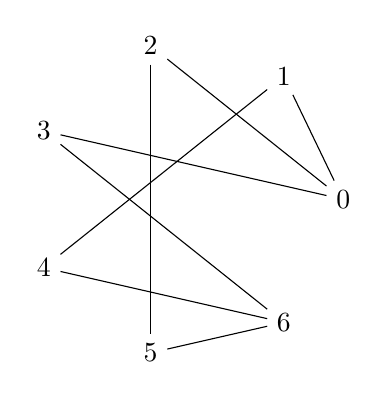
\begin{tikzpicture}
      \draw
        (0.0:2) node (0){0}
        (51.429:2) node (1){1}
        (102.857:2) node (2){2}
        (154.286:2) node (3){3}
        (205.714:2) node (4){4}
        (257.143:2) node (5){5}
        (308.571:2) node (6){6};
      \begin{scope}[-]
        \draw (0) to (1);
        \draw (0) to (2);
        \draw (0) to (3);
        \draw (1) to (4);
        \draw (2) to (5);
        \draw (3) to (6);
        \draw (4) to (6);
        \draw (5) to (6);
      \end{scope}
    \end{tikzpicture}
\end{figure}
\begin{itemize}
\item signature: 111000001000010001011
\item g: Graph with 7 nodes and 8 edges
\item order: 7
\item size: 8
\item max degree: 3
\item degrees: 2,2,2,2,2,3,3
\item is tree: 0
\item is bipartite: 0
\item has bridge: 0
\item is chordal: 0
\item is complete: 0
\item min cycle basis weight: 10
\item min cycle basis size: 2
\item diameter: 3
\item radius: 2
\item is eulerian: 0
\item is planar: 1
\item number of faces: 3
\item is regular: 0
\item p3: 11
\item p4: 14
\item property hash: cd81a1892ae78555285e740999c95a1bbf0dc8da826cc0ac1428503a025abc2a
\end{itemize}
\newpage
\begin{figure}
  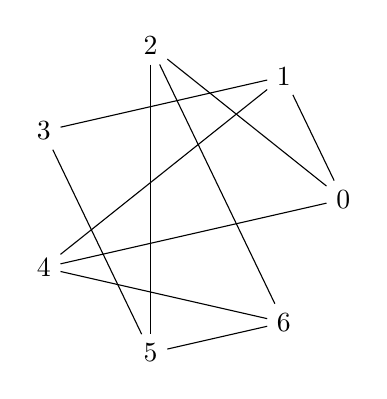
\begin{tikzpicture}
      \draw
        (0.0:2) node (0){0}
        (51.429:2) node (1){1}
        (102.857:2) node (2){2}
        (154.286:2) node (3){3}
        (205.714:2) node (4){4}
        (257.143:2) node (5){5}
        (308.571:2) node (6){6};
      \begin{scope}[-]
        \draw (0) to (1);
        \draw (0) to (2);
        \draw (0) to (4);
        \draw (1) to (3);
        \draw (1) to (4);
        \draw (2) to (5);
        \draw (2) to (6);
        \draw (3) to (5);
        \draw (4) to (6);
        \draw (5) to (6);
      \end{scope}
    \end{tikzpicture}
\end{figure}
\begin{itemize}
\item signature: 110100011000011010011
\item g: Graph with 7 nodes and 10 edges
\item order: 7
\item size: 10
\item max degree: 3
\item degrees: 2,3,3,3,3,3,3
\item is tree: 0
\item is bipartite: 0
\item has bridge: 0
\item is chordal: 0
\item is complete: 0
\item min cycle basis weight: 15
\item min cycle basis size: 4
\item diameter: 2
\item radius: 2
\item is eulerian: 0
\item is planar: 1
\item number of faces: 5
\item is regular: 0
\item p3: 13
\item p4: 14
\item property hash: 89376afab1ad6abea9eb3e0568475dca998f467a453cf71c2798508442482ca9
\end{itemize}
\newpage
\begin{figure}
  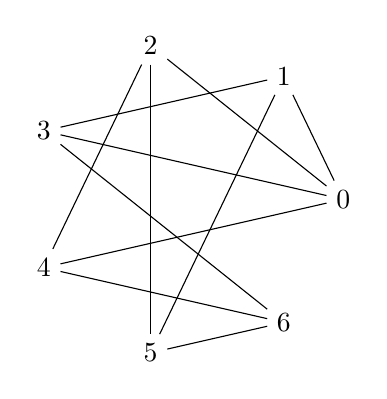
\begin{tikzpicture}
      \draw
        (0.0:2) node (0){0}
        (51.429:2) node (1){1}
        (102.857:2) node (2){2}
        (154.286:2) node (3){3}
        (205.714:2) node (4){4}
        (257.143:2) node (5){5}
        (308.571:2) node (6){6};
      \begin{scope}[-]
        \draw (0) to (1);
        \draw (0) to (2);
        \draw (0) to (3);
        \draw (0) to (4);
        \draw (1) to (3);
        \draw (1) to (5);
        \draw (2) to (4);
        \draw (2) to (5);
        \draw (3) to (6);
        \draw (4) to (6);
        \draw (5) to (6);
      \end{scope}
    \end{tikzpicture}
\end{figure}
\begin{itemize}
\item signature: 111100010100110001011
\item g: Graph with 7 nodes and 11 edges
\item order: 7
\item size: 11
\item max degree: 4
\item degrees: 3,3,3,3,3,3,4
\item is tree: 0
\item is bipartite: 0
\item has bridge: 0
\item is chordal: 0
\item is complete: 0
\item min cycle basis weight: 18
\item min cycle basis size: 5
\item diameter: 2
\item radius: 2
\item is eulerian: 0
\item is planar: 1
\item number of faces: 6
\item is regular: 0
\item p3: 18
\item p4: 14
\item property hash: 616d4a1d2541a1fb082d818ddf66bdaa1e664e52b66084f61ba2163fc56c425a
\end{itemize}
\newpage
\begin{figure}
  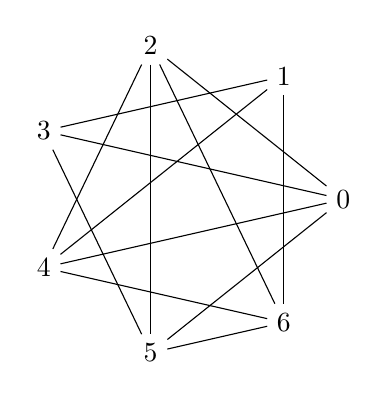
\begin{tikzpicture}
      \draw
        (0.0:2) node (0){0}
        (51.429:2) node (1){1}
        (102.857:2) node (2){2}
        (154.286:2) node (3){3}
        (205.714:2) node (4){4}
        (257.143:2) node (5){5}
        (308.571:2) node (6){6};
      \begin{scope}[-]
        \draw (0) to (2);
        \draw (0) to (3);
        \draw (0) to (4);
        \draw (0) to (5);
        \draw (1) to (3);
        \draw (1) to (4);
        \draw (1) to (6);
        \draw (2) to (4);
        \draw (2) to (5);
        \draw (2) to (6);
        \draw (3) to (5);
        \draw (4) to (6);
        \draw (5) to (6);
      \end{scope}
    \end{tikzpicture}
\end{figure}
\begin{itemize}
\item signature: 011110011010111010011
\item g: Graph with 7 nodes and 13 edges
\item order: 7
\item size: 13
\item max degree: 4
\item degrees: 3,3,4,4,4,4,4
\item is tree: 0
\item is bipartite: 0
\item has bridge: 0
\item is chordal: 0
\item is complete: 0
\item min cycle basis weight: 22
\item min cycle basis size: 7
\item diameter: 2
\item radius: 2
\item is eulerian: 0
\item is planar: 1
\item number of faces: 8
\item is regular: 0
\item p3: 18
\item p4: 14
\item property hash: e816c9acbe9b259528bf2cb1a42e3982e9ac3dd0e9a1d63fbeecb05a561dba3b
\end{itemize}
\newpage
